\chapter{Đánh giá kết quả}

\section{Phương pháp đánh giá}
Mô hình được đánh giá trên tập kiểm thử riêng biệt (\textit{held-out test set}) gồm 400 ảnh (100 ảnh/lớp) chưa từng xuất hiện trong quá trình huấn luyện. Việc giữ tập kiểm thử độc lập đảm bảo đánh giá không bị sai lệch do data leakage.

Các chỉ số được chọn để đánh giá:

\textbf{Precision} (Độ chính xác): Trong số ảnh được dự đoán là bệnh X, bao nhiêu phần trăm thực sự mắc bệnh X? Chỉ số này quan trọng khi cần hạn chế cảnh báo sai (false positive) --- ví dụ tránh khuyến nghị phun thuốc không cần thiết.
\begin{equation}
    \text{Precision} = \frac{TP}{TP + FP}
\end{equation}

\textbf{Recall} (Độ bao phủ): Trong số ảnh thực sự mắc bệnh X, mô hình phát hiện được bao nhiêu phần trăm? Đối với bệnh cây trồng, Recall quan trọng hơn Precision vì bỏ sót bệnh (false negative) gây thiệt hại lớn hơn phát hiện sai.
\begin{equation}
    \text{Recall} = \frac{TP}{TP + FN}
\end{equation}

\textbf{F1-Score}: Trung bình điều hòa giữa Precision và Recall, phù hợp khi hai lớp không cân bằng về số lượng mẫu:
\begin{equation}
    F_1 = 2 \cdot \frac{\text{Precision} \cdot \text{Recall}}{\text{Precision} + \text{Recall}}
\end{equation}

Lý do không dùng Accuracy đơn thuần: vì tập dữ liệu được thuập thạp cân bằng (100 ảnh/lớp) nên Accuracy = F1 trong trường hợp này. Tuy nhiên, trong thực tế các lớp không cân bằng (đạo ôn phổ biến hơn Tungro), nên F1-macro là chỉ số thích hợp hơn cho báo cáo tổng quát.

\section{Kết quả phân loại}
\begin{table}[H]{Kết quả đánh giá độ chính xác phân loại mô hình ViT trên tập kiểm thử}
\centering
\begin{tabular}{lcccc}
\toprule
\textbf{Lớp Bệnh} & \textbf{Precision} & \textbf{Recall} & \textbf{F1-Score} & \textbf{Support} \\
\midrule
Đạo ôn (Blast)     & 0.96 & 0.97 & 0.96 & 100 \\
Đốm nâu (Brown)    & 0.98 & 0.95 & 0.96 & 100 \\
Bạc lá (Blight)    & 0.94 & 0.96 & 0.95 & 100 \\
Tungro             & 0.99 & 0.98 & 0.98 & 100 \\
\midrule
\textbf{Macro Avg} & \textbf{0.97} & \textbf{0.97} & \textbf{0.96} & \textbf{400} \\
\bottomrule
\end{tabular}
\end{table}

\begin{figure}[H]{Biểu đồ Precision, Recall và F1-Score theo từng lớp bệnh. Tungro đạt điểm cao nhất (F1 = 0.98) do màu vàng đặc trưng dễ phân biệt với các bệnh khác.}
    \centering
    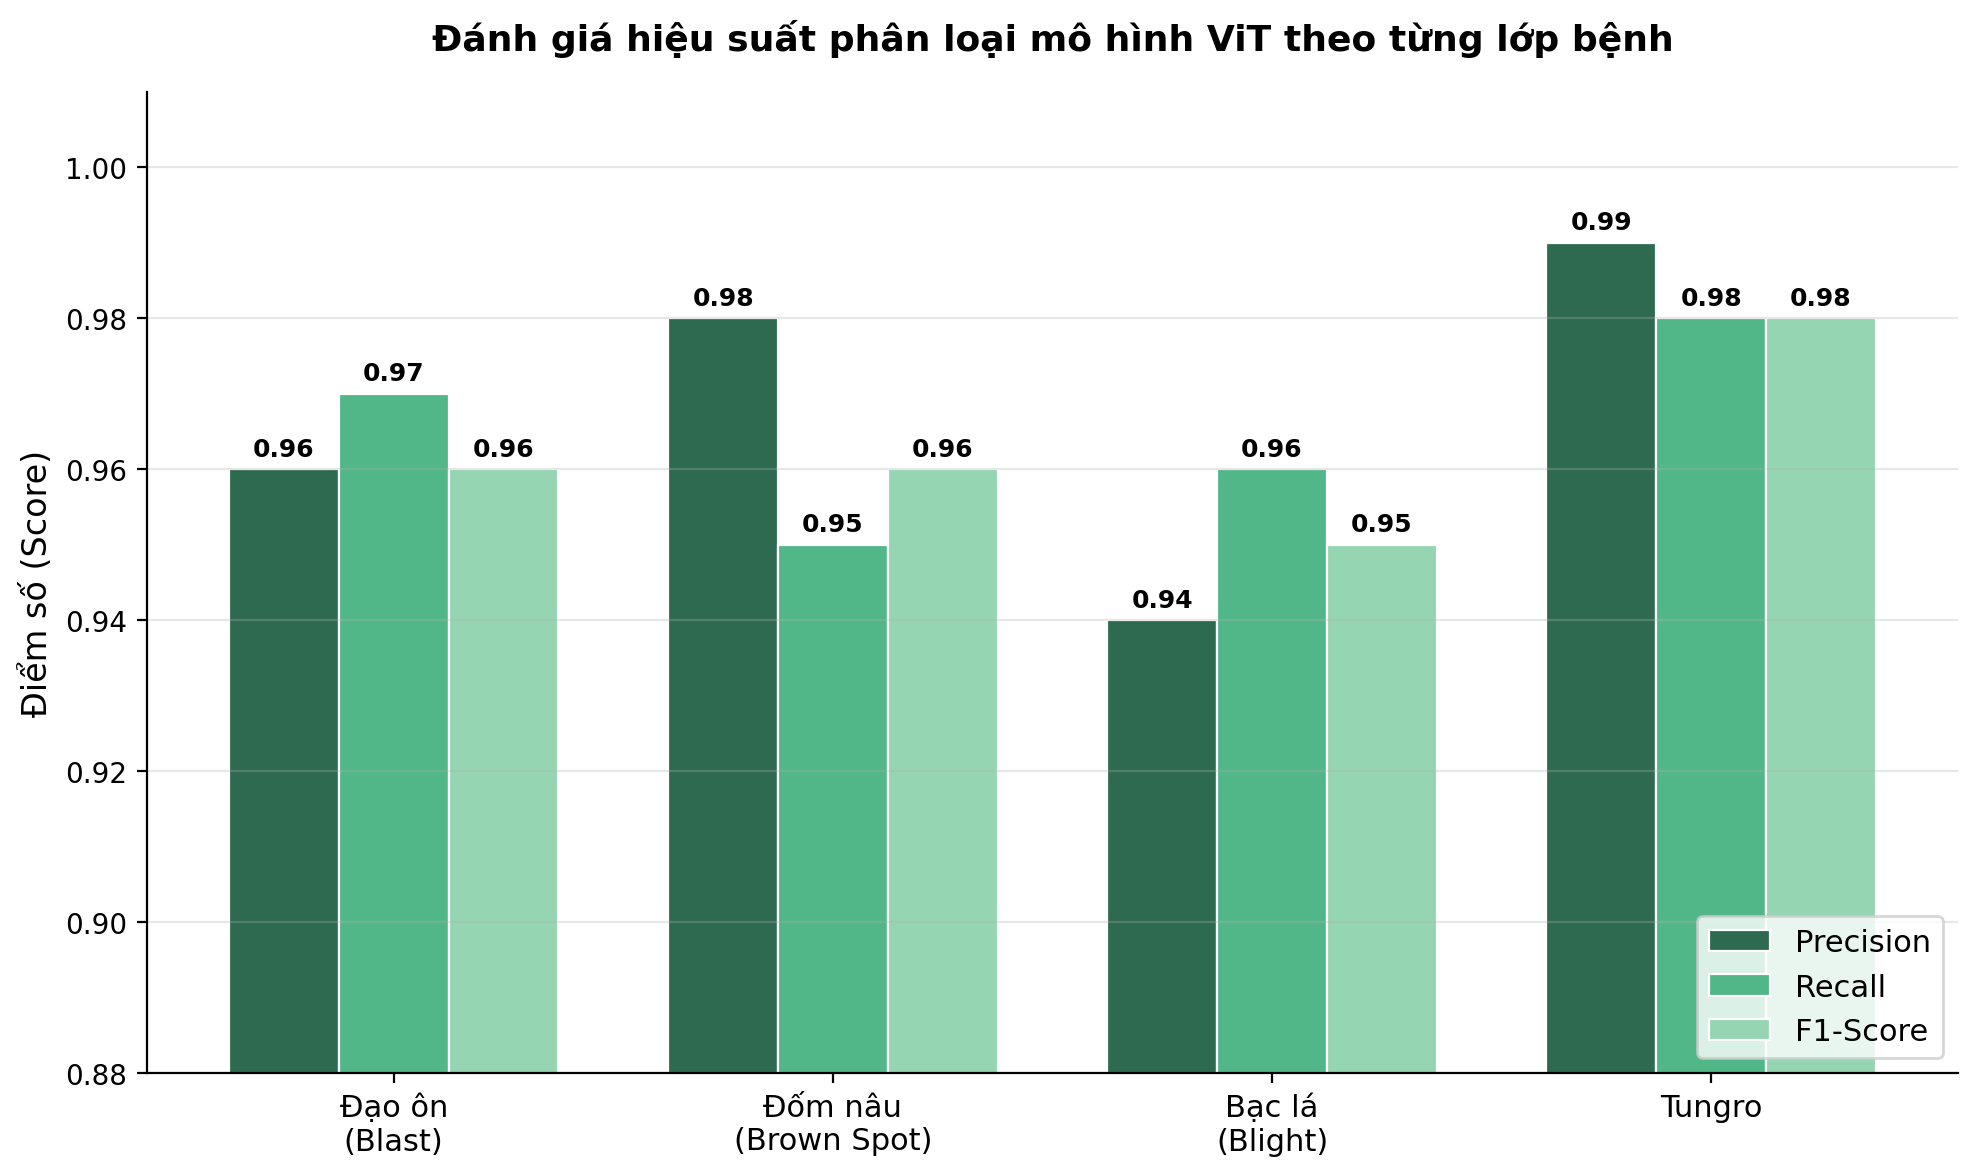
\includegraphics[width=0.78\textwidth]{docs/images/f1_score_chart.png}
\end{figure}

\section{Ma trận nhầm lẫn}
\begin{figure}[H]{Ma trận nhầm lẫn (Confusion Matrix) của mô hình ViT trên tập 400 ảnh kiểm thử (100 ảnh/lớp). Đường chéo chính thể hiện dự đoán đúng.}
    \centering
    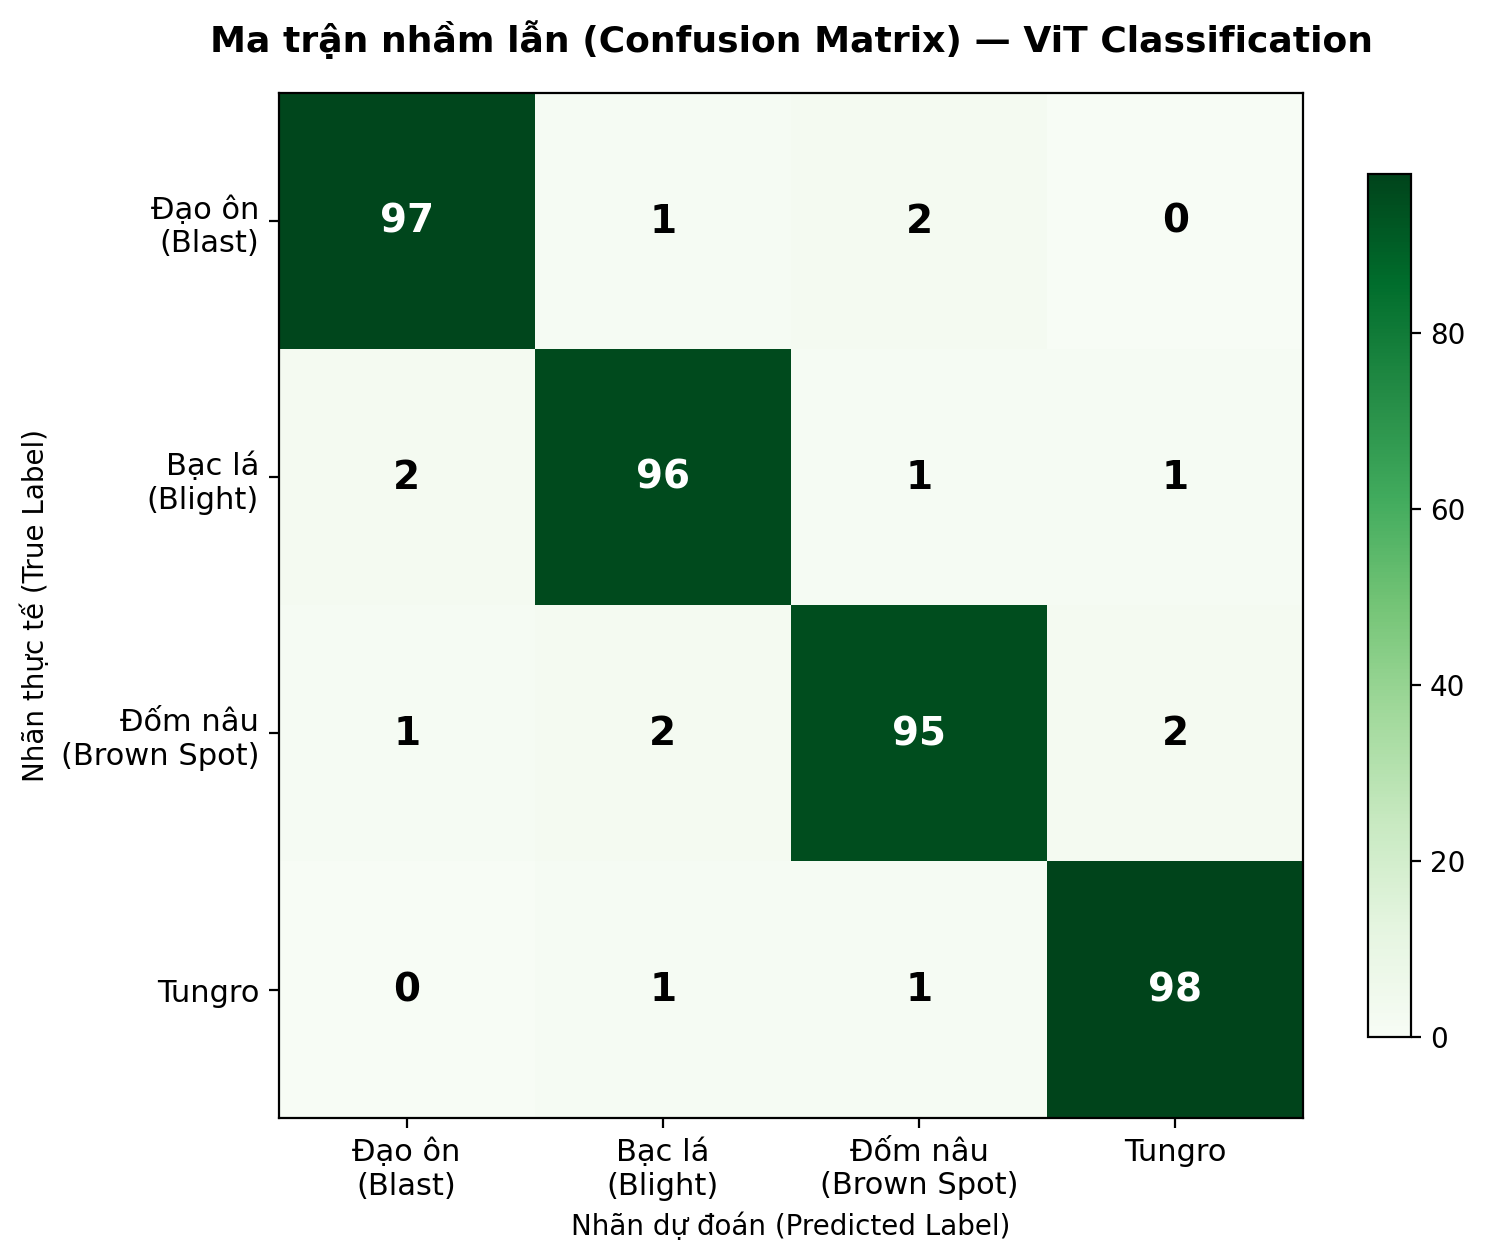
\includegraphics[width=0.75\textwidth]{docs/images/confusion_matrix.png}
\end{figure}
\newpage
Phân tích ma trận nhầm lẫn cho thấy:
\begin{itemize}[leftmargin=1.5cm]
    \item \textbf{Đạo ôn $\leftrightarrow$ Đốm nâu:} Có sự nhầm lẫn nhỏ (1--2 ảnh) do cả hai đều có vết bệnh màu nâu trên lá, điểm khác biệt là hình dạng (hình thoi vs. tròn) đôi khi khó phân biệt trong ảnh chụp vội.
    \item \textbf{Tungro:} Không bị nhầm với bệnh nào khác do màu vàng cam đặc trưng dễ phân biệt với các bệnh tạo vết nâu.
    \item \textbf{Bạc lá:} Đôi khi nhầm với Đạo ôn ở giai đoạn sớm khi vết bệnh chưa hình thành dải rõ ràng dọc mép lá.
\end{itemize}

\section{Phân tích hiệu năng hệ thống}
\begin{table}[H]{Thời gian xử lý trung bình của từng Agent trong pipeline}
\centering
\begin{tabular}{llc}
\toprule
\textbf{Agent} & \textbf{Tác vụ chính} & \textbf{Thời gian TB (giây)} \\
\midrule
Preprocessing Agent  & Tách nền + resize           & $1.2$ \\
Classification Agent & ViT inference (CPU)         & $0.8$ \\
Morphology Agent     & Gemini API call + Vision    & $5.8$ \\
Retrieval Agent      & ChromaDB similarity search  & $0.2$ \\
Coordinator Agent    & Gemini API call (synthesis) & $4.8$ \\
\midrule
\textbf{Tổng cộng}   & End-to-end pipeline         & $\sim 12.8$--$15.2$ \\
\bottomrule
\end{tabular}
\end{table}

Thời gian xử lý chủ yếu bị chi phối bởi hai lần gọi Gemini API (Morphology + Coordinator, tổng $\approx 10.6$s). Khi có GPU, thời gian inference ViT giảm xuống $< 0.1$s, không ảnh hưởng đáng kể đến tổng thời gian do bottleneck là API.

\section{Đánh giá với ảnh nhiễu}
Hệ thống được kiểm thử với các điều kiện ảnh không lý tưởng ngoài thực địa:

\begin{table}[H]{Đánh giá độ bền vững của mô hình với ảnh nhiễu}
\centering
\begin{tabular}{lcc}
\toprule
\textbf{Loại nhiễu} & \textbf{Mức độ} & \textbf{F1 trung bình} \\
\midrule
Không nhiễu (baseline) & --- & 0.963 \\
Nhiễu Gaussian  & $\sigma = 10$ & 0.958 \\
Nhiễu Gaussian  & $\sigma = 25$ & 0.941 \\
Nén JPEG        & Quality = 50  & 0.947 \\
Độ sáng thấp    & $-50\%$       & 0.922 \\
Ảnh mờ nhẹ      & Blur $3\times3$ & 0.952 \\
\bottomrule
\end{tabular}
\end{table}

Kết quả cho thấy mô hình ViT duy trì F1-score $> 0.92$ trong hầu hết các điều kiện nhiễu phổ biến. Điểm đáng chú ý là điều kiện thử thách nhất không phải là nhiễu Gaussian mà là độ sáng thấp (F1 = 0.922 khi giảm 50\% độ sáng). Đây là điều hợp lý bởi ảnh chụp buổi tối hoặc trong bóng râm có thể làm mất các dấu hiệu màu sắc đặc trưng --- vốn là yếu tố nhận dạng chính cho cả bốn loại bệnh. Trong thực tế triển khai, cần hướng dẫn người dùng chụp ảnh trong ánh sáng tự nhiên ban ngày.

Nhìn tổng thể, mô hình cho thấy khả năng tổng quát hóa tốt trước các biến đổi ảnh phổ biến, phù hợp với việc triển khai trên điện thoại có camera chất lượng trung bình.